\section{Planung der Implementierungsphase}

Die Aufgaben Implementierungsphase lässt sich grob in sechs Komponenten (Vorbereitung, Parser, Interpreter, Beweiserschnittstelle, GUI, Dokumentation) einteilen. Die ungefähre Zeitplanung und die Abhängigkeiten jedes Arbeitsschrittes sind in einem Gantt-""Diagramm~\ref{gantt_impl} verdeutlicht. Der geschätzte Arbeitsaufwand für jeden Aufgabenbereich wird in einer Tabelle~\ref{timeplan} dargestellt.

\begin{figure}
	\centering
	\hspace*{-2cm}\vspace*{-2cm}\caption[B]{Die Tasks der Implementierungsphase und ihre Abhängigkeiten}
	\hspace*{-3cm}\vspace*{-3cm}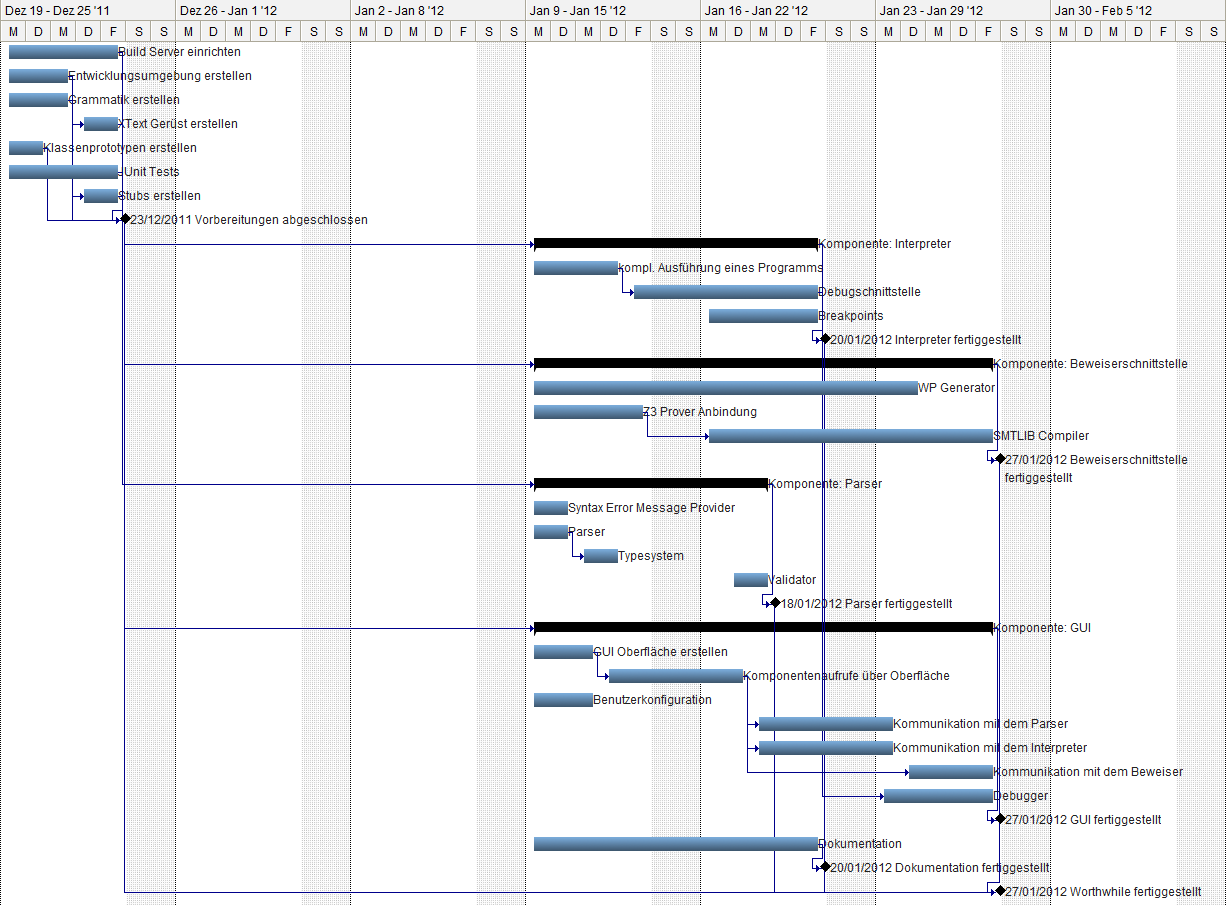
\includegraphics[angle=90,width=19cm,height= 25cm]{diagrams/gantt_implementierung_diag.png}
	\label{gantt_impl}
\end{figure}

\begin{table}[H]
	\caption[B]{Ungefähre Zeiteinteilung (in Stunden) für die Implementierungsphase}
	\label{timeplan}
	\begin{tabular}{|l|l|l|l|l|l|l|}
		\hline
		 & \textbf{Leon} & \textbf{Chris} & \textbf{Stefan} & \textbf{Joachim} & \textbf{Fabian} & \textbf{Matthias} \\
		\hline
		\textbf{Vorbereitungen} & 12 & 12 & 12 & 12 & 12 & 12 \\
		\hline
		\textbf{Interpreter} & 34 & 0 & 0 & 0 & 0 & 19 \\
		\hline
		\textbf{Beweiserschnittstelle} & 14 & 8 & 24 & 0 & 48 & 0 \\
		\hline
		\textbf{Parser} & 0 & 0 & 11 & 0 & 0 & 17 \\
		\hline
		\textbf{GUI} & 0 & 22 & 13 & 48 & 0 & 12 \\
		\hline
		\textbf{Dokumentation} & 3 & 19 & 3 & 3 & 3 & 3 \\
		\hline
		\textbf{Gesamt}	& 63 & 61 & 63 & 63 & 63 & 63 \\
		\hline
	\end{tabular}
\end{table}

\subsection{Vorbereitungen}
In der Vorbereitungsphase, welche allen anderen Arbeitsschritten voranliegt, wird hauptsächlich das Klassendiagramm in Quelltext umgesetzt sowie eine Basis für die Implementierungen eingerichtet. Hierzu gehört insbesondere das Erstellen der Grammatik für die WHILE-Sprache und das Ausrüsten aller Komponenten mit Stubs, um eingeschränkt funktionierende Schnittstellen für die anderen Teile des Programms bereitzustellen. Desweiteren werden JUnit-""Tests erstellt, die implementierungsbegleitend benutzt werden sollen. Durch die vorgesehenen Stubs müssen alle JUnit-""Tests erfolgreich ausgeführt werden können. Die Integration der einzelnen Komponenten erfolgt durch Austausch des betreffenden Stubs. Im Verlauf der Implementierungsphase wird Wert darauf gelegt, dass ein Stub nur dann gegen eine funktionierende Schnittstelle ausgetauscht wird, wenn gewährleistet ist, dass der zuständige JUnit-""Test immer noch erfolgreich abläuft. In dieser Phase werden alle Mitglieder des Teams in etwa gleich beansprucht. Nach erfolgreicher Beendigung der Vorbereitungen können die Arbeitsabschnitte für die jeweiligen Komponenten des Projekts (Interpreter mit Run-""time-""Checker, Beweiserschnittstelle, GUI) anlaufen.

\subsection{Parser}
Möglichst frühzeitig wird die Parserfunktionalität soweit erstellt, dass das Parsen ohne semantische Prüfung eines Programms möglich ist. Dieser Teil ist von hoher Wichtigkeit, da hierdurch das übrige Projekt auf aus beliebigen Programmtexten erstellte Abstract-""Syntax-""Trees~(AST) zurückgreifen kann und nicht mehr nur der Stub-AST verwendet werden muss. Somit können frühzeitig Mängel am Modell des Abstract-""Syntax-""Tree erkannt werden. Anschließend kann die Einbindung des Typsystems erfolgen und die Funktionalität des Validators aufgenommen werden.

\subsection{Interpreter}
Zu Beginn dieser Arbeitseinheit erfolgt die Implementierung der Grundfunktionalität des Interpreters. Die komplette Ausführung eines durch einen AST spezifizierten Programms soll ermöglicht werden, um Fehler des vom Parser erzeugten ASTs frühzeitig zu erkennen. Anschließend wird die Debugschnittstelle entwickelt, deren Funktionalität wichtig für das Testen der GUI während deren Entwicklung ist. Die Einbindung der Unterstützung für Breakpoints kann parallel hierzu erfolgen.

\subsection{Beweiserschnittstelle}
In dieser Arbeitseinheit ist der Teil für die Generierung der Weakest-""Precondition unabhängig von der Anbindung des Beweisers und des Compilers für die SMTLIB-Sprache und kann somit parallel hierzu bearbeitet werden. Die Übersetzung von Formeln in SMTLIB ist abhängig von der Anbindung des Beweisers, da es hiermit ermöglicht wird, den SMTLIB-Compiler zu testen und damit auch korrekt zu implementieren.

\subsection{GUI}
Die GUI kann in vielen Bereichen unabhängig vom Rest des Projekts entwickelt werden. Es ist jedoch von Vorteil die Kommunikation mit den einzelnen Komponenten erst dann zu implementieren, wenn eine gewisse Grundfunktionalität der jeweiligen Komponente gegeben ist. Deshalb wird die Oberfläche der GUI sowie die Benutzerkonfigurationskomponente zu Beginn erstellt. Anschließend kann parallel zu der Implementation der von der GUI benötigten Schnittstellen in den anderen Komponenten die entsprechende Funktionalität in der GUI eingefügt werden. Der Debugger wird entwickelt, sobald der Interpreter fertiggestellt ist.

\subsection{Dokumentation}
Die Dokumentation besteht aus einem ausführlichen Benutzerhandbuch, einer Schnittstellendokumentation sowie Beispielprogrammen. Sie wird zu Beginn der Implementierung der anderen Komponenten begleitend erstellt und laufend aktualisiert, um Konsistenz und Vollständigkeit zu sichern. Bei dieser Komponente wird jedes Teammitglied, überwiegend in seinem zugehörigen Bereich, beteiligt sein.
